The multivariate shape analysis gives the best sensitivity in computing the upper limits, 
as shown in Section~\ref{sec:results} and Section~\ref{sec:dataresults}. 
The inputs to the limits are the binned histograms of the multivariate discriminant for 
data and the backgrounds.  
In the current implementation of LandS~\cite{lands} package, 
the statistical uncertainties associated with the background template 
can only be included as the uncertainty of the overall expected yields.  
As the statistical uncertainty at each bin is larger than the overall uncertainty, 
this simpfied approach could lead to an overestimated limit. 
The exact impact depends on the size of the background samples from which 
the background template is built upon. 

To account for the bin-by-bin statistical uncertainties and estimate
the effects on the measured upperlimits shown in
Section~\ref{sec:dataresults} we use the following procedure. Instead
of using the histograms directly as an input to the LandS calculation,
we write out an input card for each bin in which the correct
statistical uncertainty is used. We then combine these cards to
compute the upper limits. If the background template at a given bin is
empty, we flucturate the bin content equal to one even count and
assign 100\% relative uncertainty.  The results obtained this way is
then compared with the default shape analysis results to evaulate the
effects, as tabulated in Table~\ref{tab:shapeuncertain}.

This method provides full systematic uncertainty evaluation for the
shape analysis since the uncertainty on the shape is taken directly
from data driven background estimation and the uncertainty is properly
taken into account.

%%%%%%%%%%%%%%%%%%%%%%%%%%%%%%
\begin{table}
\begin{center}
\begin{tabular}{c c c c c c c c c c c c c}
\hline
 $m_H$ (GeV) & 115 & 120 & 130 & 140 & 150 & 160 & 170 & 180 & 190 & 200 & 250 & 300 \\
  diff (\%) & 0.6 & -0.2 & -2.0 & -0.2 & 3.6 & -0.4 & 4.7 & 1.9 & 1.2 & 2.2 & 0.0 & -1.1 \\
\hline
\end{tabular}
\end{center}
\caption{Effect of including the bin-by-bin statistical uncertainties. The difference is calculated as the 
relative difference in the median of the expected limits at 95\% C.L. correponding to 200/pb  
between the results obtained including the bin-by-bin uncertainty and the results obtained 
from the default shape analysis. }
\label{tab:shapeuncertain}
\end{table}

As a cross-check, we show the multivariate output distribution for top-tagged and non 
top-tagged simulated events in Figure~\ref{fig:mva_top}.

%%%%%%%%%%%%%%%%%%%%%%%%%%%%%%
\begin{figure}[!htbp]
\begin{center}
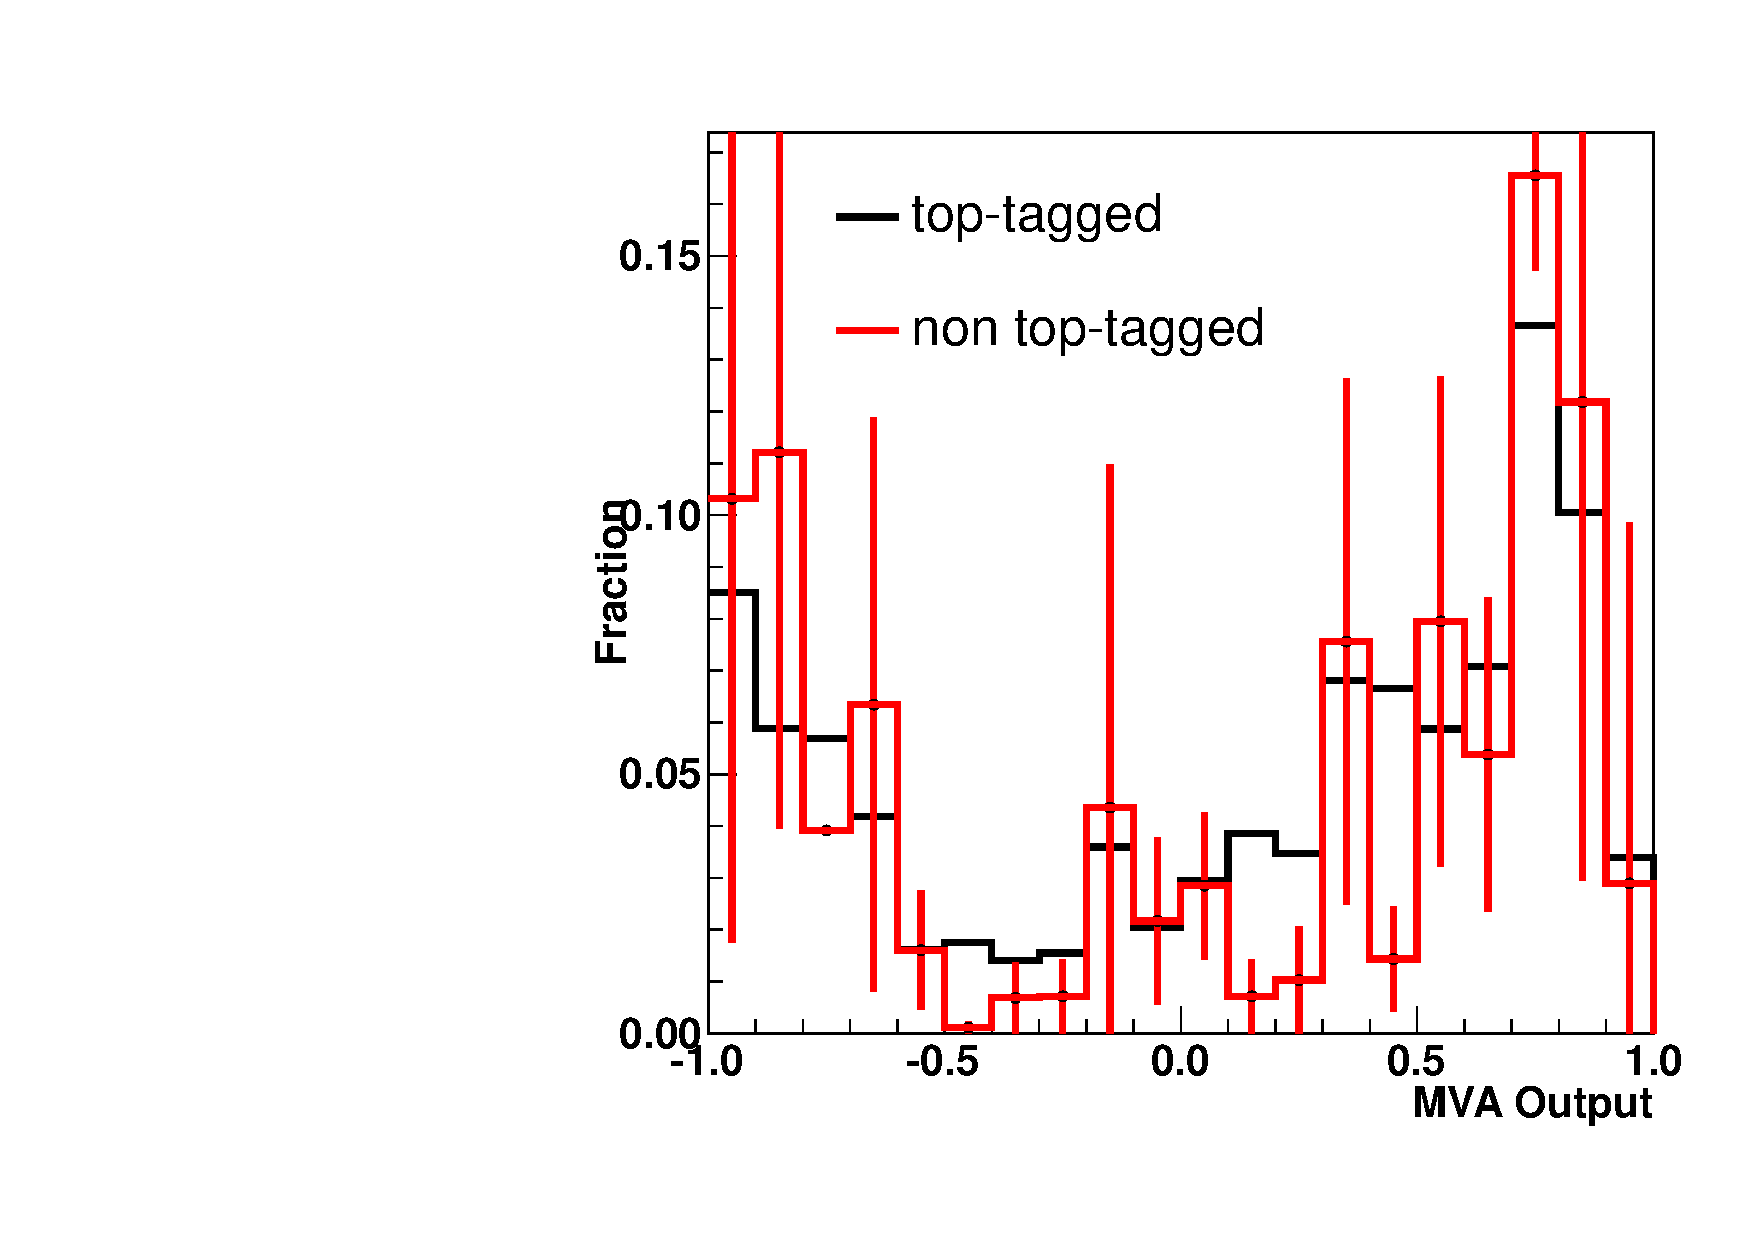
\includegraphics[width=0.7\textwidth]{figures/mva_top.pdf}
\caption{Multivariate output distribution for top-tagged and non top-tagged simulated events.}
\label{fig:mva_top}
\end{center}
\end{figure}
%%%%%%%%%%%%%%%%%%%%%%%%%%%%%%



 
